\documentclass[article,type=msc,colorback,12pt,accentcolor=tud7b,table]{tudthesis}
%\usepackage[table,xcdraw]{xcolor}
\usepackage{ngerman}
\usepackage[english]{babel}
\usepackage{cite}
\usepackage{hyperref}
\usepackage{float}
\usepackage{listings}
% If you use beamer only pass "xcolor=table" option, i.e. \documentclass[xcolor=table]{beamer}
\graphicspath{ {images/A/} {images/B/} {images/C/} {images/D/}{images/E/}}

\hypersetup{
    colorlinks,
    citecolor=blue,
    filecolor=blue,
    linkcolor=blue,
    urlcolor=blue
}


\newcommand{\getmydate}{%
  \ifcase\month%
    \or Januar\or Februar\or M\"arz%
    \or April\or Mai\or Juni\or Juli%
    \or August\or September\or Oktober%
    \or November\or Dezember%
  \fi\ \number\year%
}

\begin{document}
  \thesistitle{Feedback Driven Development of Cloud Applications} 
  %\linebreak[1]Corporate-Design f"ur {\LaTeX}!}%
    {Feedback Driven Development of Cloud Applications}
  \author{Harini Gunabalan}
  \birthplace{}
  \referee{Prof. Dr.-Ing. Mira Mezini}{Dr. Guido Salvaneschi, Dr. Gerald Junkermann, Aryan Dadashi}
  \department{Department of Computer Science}
  \group{Software Technology Group}
  \dateofexam{31 May 2015}{31 May 2015}
  \tuprints{12345}{1234}
  \makethesistitle
  \affidavit{Harini Gunabalan}
\cleardoublepage

\section*{\begin{center}
		{\huge Acknowledgment}
	\end{center}}
	\vspace*{\fill}
	\begin{center}
		\par \textit{"Thanks to Guido, Gerald, Aryan, Juergen, Anne, Prof. Mezini, Hari and friends for playing a major role in supporting my Master Thesis work."}\\
		\begin{flushright}
			\textit{	-Harini}
		\end{flushright}
	\end{center}
	\vspace*{\fill}
	\clearpage


\begin{abstract}
\begin{large} 
	
	Over the last few years, the Cloud Computing Paradigm has gained a lot of importance in both the Academia and the Industry. The cloud has not only changed the IT Landscape from the user's perspective but has also changed how the Developers develop applications on the cloud and how the Operators have to automate provisioning Infrastructure. The increasing adoption of the DevOps approach has led to the removal of the boundaries between the development and the operations. 
	\leavevmode
	\newline

	Among the the three levels of the Cloud Computing: Infrastructure-as-a-Service (IaaS), Platform-as-a-Service(PaaS) and Software-as-a-Service(SaaS), Software Developers are mainly concerned with the PaaS which allows them to focus on the Application Development. Leveraging the fact that the Application is hosted on the cloud, there are additional metrics regarding the application available to Developers in different Log formats. There are also Cloud Monitoring Tools which consolidates these logs with a huge volume of data representing the run-time metrics etc. of the cloud applications. Though monitoring of the cloud applications has been done by many tools, most of the DevOps do not go through the cumbersome error/warning log data. Utilizing this information, it is possible to have an overview of the Application Performance at real time. This aids in capturing issues that occur at scale which normally could not be captured by Profilers. This could also help us to reduce the developer-operator gap providing an improved DevOps experience. 
	\leavevmode
	\newline

	This thesis work makes use of the monitoring data to implement a platform level AutoScaler. Developers can continue to deploy new features and operators do not have to manually intervene into deploying more application instances as the application scales.
	
\end{large}
\end{abstract}  

\clearpage

%=====INDEX================================================================================
\setlength{ \parskip }{1em}
\index{key}
\tableofcontents 
\cleardoublepage 
\listoffigures
\cleardoublepage 
\listoftables
\clearpage
\appendix
\cleardoublepage 

% abstract, acknowledgements, contents
 \section{Introduction}
	
	Cloud Computing is one of the fields in Computer Science that has gained rapid growth and importance in the recent years. The fact that the servers are remote hosted rather than local servers has led to innumerable small scale businesses. Start-ups no longer require high infrastructure, instead they just need to pay for the amount of resources that they actually use (pay-per-use). This also significantly reduces the initial monetary setup costs for such start-ups. There has been extensive research in Cloud Computing areas such as auto-scaling of resources at the infrastructure level, monitoring of metrics at both the application and infrastructure level. However, there is not much research done in how these monitored metrics are utilized by the Cloud Application Developers. Making the run-time metrics visibly effective for the developers in their Development Environment is the issue this thesis is aiming to solve.
	\par This chapter is structured into four sections. The first section provides the motivation of this thesis work. The second section gives an insight into the problem statement which this Thesis work aims to solve. The third section details the contribution of the work and the fourth section provides how the following chapters of the Thesis are structured.
	
	\subsection{Motivation}
	
	Software Engineering Practice in the industry has faced a phenomenal change since the advent of Cloud Computing. This is mainly due to the flexibility and the dynamic scaling up and scaling down of the infrastructure as required by the current workload. This proves not only to be elastic but cost-effective as well. It is quite obvious that this elasticity is achieved by the continuous monitoring of several metrics that indicate the demand at the moment, and provisioning the necessary resources to meet the monitored demand. Distributed, scalable enterprise-wide applications also mandate the monitoring of metrics for reasoning the effectiveness of the applications by engineers and business analysts \cite{leitner2012application}.
	
	\par The metrics that are being monitored vary widely. For instance, the metrics such as memory consumption, CPU utilization, Network bandwidth utilization could be considered to be at the Infrastructure level, whereas some other metrics such as Response times of methods/procedures, the number of users accessing the application, maximum number of users who can use the application simultaneously, etc. could be considered to be at the application level. Sometimes, the application level metrics could depend on the primitive metrics at the infrastructure level and vice-versa.
	
	\par As Cloud Application Development has becoming more common, the run time monitoring metrics of these applications are available through several Application Performance Monitoring (APM) tools such as Amazon Cloudwatch, New Relic, etc. But, they do not provide any valuable and visible feedback to the developers, and hence most of the cloud developers do not use it. However, this run-time monitoring data could be used to provide useful analytic information such as performance hotspots that is taking a lot of execution time, and predictive information such as methods or loops that may become critical, even before the deployment. This type of analytic and predictive feedback should be provided to the developers in their IDEs which otherwise may not be explored by the developers. This technique of utilizing the monitoring data is known Feedback driven development. Feedback Driven Development that provides visual tools to the cloud developers is the focus of this thesis research.	
	
	\subsection{Problem Statement}	
	
The Cloud computing paradigms are classified into three service models which forms a stack as shown in Figure 1. The three layers work coordinate with each other.

 \begin{figure}
 \begin{center}
  \makebox[\textwidth]{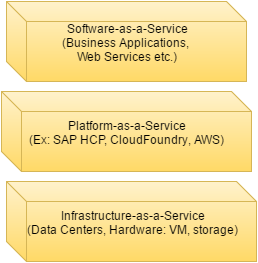
\includegraphics[scale=0.7]{A1}}
\end{center}
\caption{Cloud Computing Stack}
\end{figure}

%\begin{itemize}
%	
%	\item Infrastructure-as-a-Service
%	
%	\item Platform-as-a-Service
%	
%	\item Software-as-a-Service  
%% add the stack image 	
%\end{itemize}
	
\cite{bruneo2015framework} defines a framework that collects data as defined by a 3-D cloud monitoring model. From the software engineering perspective, it is important to note how Cloud Computing impacts the development practices. Based on the research conducted, there are two important research issues \cite{cito2014making}. 

\begin{itemize}

	
	\item Impact of DevOps on Cloud Application Developers:	
	The Cloud Developers are forced to look into the huge log data of the cloud applications. Development and Operations are brought much closer than the traditional software methods. Sometimes the same person acts as both the developer and the operator. 
	
	\item Data and Tools utilized by Cloud Developers:
	The data produced by the logs include Business Metrics, System-level Data etc. Sometimes the implementation changes may even have monetary consequences in the cloud, nevertheless most of the developers do not pay attention to this aspect. Hence it can be argued that once these operational metrics are brought closer to the Cloud Developers Environment, they would be able to pay closer attention to this information thereby achieving cost-effective applications.
	
\end{itemize}

Considering these issues, it is certainly important how we are going to leverage these Cloud monitoring Logs to make a useful impact for the Cloud Developers and Cloud Operators. 
 
 	\subsubsection{Continuous Delivery in Cloud Development}
 	As we compare the software development on-premise with that of the Cloud, there has been a huge change in every software release. Deployment cycles has been reduced from months to days and sometimes even within a few hours the next version is released. This process is often referred to Continuous Delivery(CD) in the Cloud Computing terms. Most companies make use of this Continous Delivery to rollout new features and evaluate their new ideas in a controlled manner \cite{kohavi2007practical}. CD has become a huge success and companies such as Google,Facebook etc. adopt CD of varying degrees for some of their services. When a feature is delayed for the current roll-out, it gets delayed by months when the traditional software development life-cycle is used. The feature needs to be delayed until the next release. Whereas in this CD approach the next release could be in the same day or in the same week, leading to small changes of production code. This also leads to a state called "perpetual development" where the code is always under continuous development and there is no stable release version for a particular product.  	\par Owing to this new release paradigm, there are a lot of extra information generated. The live performance of the application, click-streams from the User Interface of application, error and warning logs, infrastructure related data etc. are produced. There are a lot of existing APM Tools that collect this data and generate information out of it, however, how this information could be made effective to the software developers or cloud operators in their daily routine is a topic that is not discussed very often. 
 	
 	\subsubsection{Monitoring Metrics: Scalability and Availability of the Application}
 	
	Some of the monitoring metrics collected include the CPU usage, response time of the request, number of instances the application is hosted on, no. of requests each instance serves during a particular time period, error logs of the request etc. While these metrics focus mainly at the Infrastructure level, the logs instrumented into the application are also collected. We use these metrics to focus on two main challenges of cloud computing: Scalability and Availability of the Cloud applications.
	
	\par Scalability is the ability to increase or decrease the resources of an instance or the number of instances so that the changing demand of the incoming requests can be met. The platform related log data are collected for both Horizontal scaling (increasing the number of instances) and Vertical scaling(increasing the resources of each instance).
	
	\par Availability is one of the major goals of Cloud Computing. It means that the Cloud Services need to be available and accessible at anytime from anywhere. For business to happen continuously, it is necessary for the services to be highly available. The definition of availability is specified by the different Cloud vendors in their SLAs. For example, Google Search is known for its high availability.	
	
	\subsubsection{Incorporating the collected Feedback for Operations}	
	
	Using the collected metrics, in this thesis, we aim to provide an efficient feedback to the Cloud Operators. In \cite{cito2015runtime}, the collected feedback is integrated into the Development Environment (IDEs) so that developers are able to utilize the feedback to make their applications better scalable and highly available. This feedback can also be leveraged to automate configuration management to facilitate dynamic Infrastructure Provisioning.
	
	\subsection{Dissertion Roadmap}

	\par This thesis is structured in six chapters. Chapter 1 provides a short introduction into the topic and describes the goals of the thesis. Chapter 2 includes more background information and presents the state of the art of the important topics of this thesis: Cloud Application Performance Monitoring(AMP) tools, Feedback Driven Development(FDD) in general, and how FDD could be useful for Cloud Application Developers. The third Chapter describes an overview of the high-level System Design and the design decisions made in this research work. The fourth chapter explains the system on a lower fine-grained level. Interesting Implementation details are also provided here. Chapter 5 shows the various case studies, evaluates the developed system and illustrates its usage as well as possible applications. Finally, Chapter six provides the conclusion of the thesis and outlines the future work ideas.

% Example of Footnote    
%     \textbf{Alle Vordefinierten Texte sind, wie verbindlich vorgeschrieben, in der hessischen Amtssprache
%    gehalten\footnote{Deutschland hat (noch) keine Amtssprache.}.}

	\cleardoublepage

 \section{State of the Art}
 	
	This chapter presents the state of art of the topics relevant for this thesis. In the first section, we explain what is Feedback Driven Development(FDD) and the types of FDD. The second section briefs about Auto-scalers and third section provides a background on Data Modeling. The fourth section describes about mining source code changes to identify performance regressions and the final section details about . 
	
		\subsection{Feedback Driven Development } 		
		
		By analyzing any Cloud Application's logs, we can get hold of a huge amount of information. This can be broadly classified into: Application Level Logs and Infrastructure Level Logs. This data could be made useful to both the Developers and Operators. Infrastructure Logs provides details such as number of instances, the memory, CPU, Disk utilization of each instance, which instance serves a particular request etc. By making this kind of data visible to the developers, they can tweak the application development process, as they have access to the cloud internals. At the same time, the Cloud operators also benefit with the relevant business metrics to manage the instances more efficiently. 
		
		\par Collecting these run-time data, aggregating them into useful feedback, and feeding them back into the Development process of an application could create a useful impact in the future deployment of the application. This process is known as Feedback Driven Development(FDD). FDD can be classified into 2 types: Analytic FDD and Predictive FDD \cite{cito2015runtime}.
		
		\begin{itemize}
			\item{Analytic Feedback Driven Development: }
			Analytic FDD is the run time data from the previous deployments, which is brought directly into the developer environment. It provides a mapping between the log data collected and the source code artifacts. This helps the developers to understand how the run-time metrics directly impact the source code. Based on this developers can alter and optimize the code based on the real time user behavior. In practice, Analytic FDD deals with visualizing the run time operations data and how it is being mapped to the code artifacts. 
			
			\item{Predictive Feedback Driven Development: }
			Predictive FDD is one step ahead compared to the Analytic FDD. It utilizes the run-time feedback to warn the developers about the current code changes even before the updated source code is deployed. Predictive FDD is combined with static code analysis to give better predictions regarding a code change. 
		\end{itemize}
	
	\subsection{Cloud Monitoring}
 	
 	As Cloud Computing is gaining popularity, the need for Cloud monitoring is becoming increasingly important to  both the Cloud Providers and the Cloud Consumers. At the Cloud Provider side, Cloud Monitoring is the key principle behind which the actual controlling of hardware takes place. It enables them to scale the infrastructure, if necessary. On the Cloud Consumer side, Cloud Monitoring enables to check the Availability, QoS etc. of the applications. The consumers can verify any SLA violations by comparing the Key Performance Indicators(KPI) parameters provided by Cloud Monitoring.
 	
 	\cite{aceto2013cloud} explains in detail about the need for Cloud Monitoring: the basic concepts involved, the properties which needs to be maintained, and finally also lists down the open issues with respect to Cloud monitoring. These are summarized in Figure 2.
	
	There are several Cloud monitoring platforms and services such as CloudWatch \cite{cloudwatchdev} \cite{cloudwatch}, AzureWatch \cite{azurewatch} , NewRelic \cite{newrelic} etc. Table 1 provides a list of Cloud Monitoring platforms and services. Amazon CloudWatch provides users the monitored information for 2 weeks. Users are allowed to plot these information, set thresholds, alerts etc and these alerts can be used to perform any substantial action such as sending an Email or even in AutoScaling \cite{aas}. AutoScaling is explored in detail in the next section. 
	
\begin{table}[h!]
  \centering
  \caption{Cloud Monitoring Platforms and Services }
  \label{tab:Table1}
  \begin{tabular}{l|l}
  \hline
  \rowcolor[HTML]{FFCB2F}  \textbf{Cloud Monitoring Platforms}  & \textbf{Cloud Monitoring Services} \\
    \hline
    CloudWatch \cite{cloudwatchdev} \cite{cloudwatch} & New Relic \cite{newrelic} \\    
    Nimsoft \cite{nimsoft} & Cloudyn \cite{cloudyn} \\        
    AzureWatch \cite{azurewatch} & Up.time \cite{uptime} \\        
    Nagios \cite{nagios} & CloudSleuth \cite{cloudsleuth} \\
    Nimbus \cite{nimbus} & Cloudstone \cite{cloudstone} \\ 
    GroundWork \cite{groundwork} & Boundary \cite{boundary} \\
    LogicMonitor \cite{logicmonitor} & Cloudfloor \cite{cloudfloor} \\ 
    CloudKick \cite{cloudkick} & CloudClimate \cite{cloudclimate} \\    
    Monitis \cite{monitis} & CloudHarmony \cite{cloudharmony} \\
    \hline
    
  \end{tabular}
\end{table}
	
	Some other Cloud Monitoring Platforms such as Nimsoft Monitoring Solution \cite{nimsoft} provides a unified monitoring dashboard to view infrastructures provided by Salesforce, Rackspace, Google or Amazon. Nagios \cite{nagios} is a popular open source Cloud Monitoring platform which provides monitoring of virtual machines and storage (Amazon EC2 and S3). It also supports OpenStack \cite{openstack}, an open Source Cloud IaaS. New Relic \cite{newrelic} is a web-based Monitoring service that helps to monitor the application infrastructure and performance, adhering to timeliness, resilience, availability and accuracy.
	
	While all of the above Cloud Monitoring platforms and services are great, most of them do not consider multiple layers or real-time data. Some of them consider multiple layers whereas do not take into account the real-time data, and some consider real-time data but do not consider the multiple cloud layers \cite{marquezan20143}. \cite{bruneo2015framework} proposes a 3D-Cloud Monitoring framework called the Ceiloesper framework, which combines monitoring in multiple layers with real time data and it also performs the data analysis for multiple management actions. It is based on the Complex event processing (CEP) and uses the Esper CEP Engine.
 		
%	\subsection{Logging}
%		
%		As depicted in \cite{jiang2009understanding} , it is clear that Auto Generated issues are resolved much faster than human generated issues. Auto generated issues are those that have attached symptoms and system logs as event messages, whereas Human generated issues are those reported by the users usually through email tickets/phone calls. This further justifies the use and necessity of logging. \cite{jiang2009understanding} also lists down the challenges of using the logging information.
%		
%		The Log Data collected to generate the feedback is discussed here. Among the two types of data: Monitoring Data and Production data as detailed in \cite{cito2015runtime} we focus on the Monitoring data. This category of data is further classified as Load Data (incoming requests, server utilization, number of instances), Performance data (Response times, hotspots), cost data and User Behavior Data (Click Streams). This data is mostly collected by existing APM Tools.
%		
%		\cite{yuan2012conservative} answers the question of where to add logs proactively that could help minimize the effort of failure diagnosis. ERRLOG, a tool that identifies in which location log needs to be added is developed. Errlog makes use of code analysis techniques to achieve this. iTrack, a framework for monitoring user activities and correlating them with system data is done to detect service outages as in \cite{mann2011correlating}. 
%			
%	\subsubsection{Logging Tools and Metrics}	
%
%		\subsubsection{Log Structure}	
%		
%		\subsubsection{Performance related Logging}
%		\cite{nagaraj2012structured} explains a tool known as DISTALYZER that analyses the system logs to identify the performance issues. This tool analyses logs from large scale distributed systems and compares a set of baseline logs with an acceptable performance with another set of logs with unacceptable performance. DISTALYZER uses machine learning techniques which first creates a set of features(event/state variables) for the logs. Further Predictive and Descriptive Modeling are performed on these variables to provide the developers the root cause of the issue.
%
%		\subsubsection{Click Stream Logging}
	

\begin{figure}
 \begin{center}
  \makebox[\textwidth]{\includegraphics[width=\textwidth]{B5}}
\end{center}
\caption{Cloud Monitoring \cite{aceto2013cloud}}
\end{figure}	
	
	\subsection{Auto-scaling}	
	
	Scaling of Cloud Infrastructure means changing the current infrastructure. It could be of two types: Horizontal and Vertical Scaling. Horizontal Scaling is a methodology of adding/removing machines whereas vertical scaling is increasing/decreasing the resources such as CPU/Memory/Disk to existing machines.
	
	The Metrics monitoring and Data Collection has a huge importance with respect to Auto-scaling. Auto-scaling or automatic scaling is a process where the Cloud Platform adapts itself by increasing or shutting down the number of instances on which the application is currently deployed depending on the current load. For enterprises running their own infrastructure shutting down servers that are not being utilized could save electricity costs, whereas for enterprises running their applications on Cloud, auto-scaling could lead to saving costs due to the pay-per-use model of the Cloud. Auto-scaling also improves the efficieny of applications. In the scenario mentioned in \cite{bunch2012pluggable}, auto-scaling improves the instance utilization of the open source AppScale PaaS by 91\% and it also brings down the average time taken to serve the requests. Auto-scalers can be broadly classified as the following: 
	
	\begin{itemize}
	
	\item{Reactive Auto-scaling: }Auto-scaling as provided by most of the cloud providers such as Amazon Web Services, Microsoft Azure, and IBM Bluemix etc are reactive. This means based on monitoring the relevant metrics, whenever a certain metric increases or decreases beyond a particular predefined threshold, additional instances are added or removed. This method which is more of a rule-based mechanism is a reactive auto-scaling method. This is easier to be implemented as it involves monitoring metrics, and framing rules and policies for scaling. While this method serves in most scenarios, the question arises whether it is capable to handle bursty traffic.
	
	In \cite{seelam2015polyglot} the rule based reactive autoscaler of IBM's Bluemix PaaS, Polyglot application, is described. Polyglot autoscaler allows application developers to set thresholds based on which instances need to be added (scale-out) or removed (scale-in). These threshold values could be parameters such as CPU Utilization, memory and heap usage. The architecture of the Polyglot autoscaler can be found in Figure 3. It consists of the four components: Agents which collect the performance information, a monitoring service which continuously monitors the health of the cloud application, a scaling service which makes the decision of whether scaling needs to be performed or not, and a Persistence service to keep track of the enactment points (points where the application is scaled in time).  

\item{Predictive Auto-scaling: }Predictive auto-scaling comes very handy to handle bursty workloads. By analyzing the historic time series data, it may be possible to predict the workload at a future time, thereby enabling predictive auto-scaling. The effectiveness of this method depends on the efficiency of the workload prediction.

\cite{biswas2015predictive} introduces a predictive auto scaling technique that uses a Machine Learning engine to make predictions based on a deadline driven algorithm for predicting the future state of the system. \cite{Scryer1} and \cite{Scryer2} describes a predictive auto-scaling tool, Scyer, used by Netflix to provision the correct number of Amazon Web Services \cite{aws} instances. This is different from the Amazon AutoScaling(AAS) \cite{aas}, which is a reactive one. Scryer's prediction engine is able to provision the resources based on two prediction algorithms to predict the workload. The prediction algorithms implemented are augmented linear regression based algorithm and Fast Fourier Transformation based algorithm.

\item{Hybrid Auto-scaling: } Hybrid Auto-scaling is a combination of both the Reactive and Predictive approaches. As mentioned in \cite{Scryer1}, Scryer tool works in co-ordination with the AAS for more efficient auto scaling. \cite{moore2013coordinated} describes the architecture and implementation of Platform Insights, which is another hybrid auto-scaler that employs a reactive rule-based and a predictive model-based approach in a coordinated manner.
\end{itemize}
Auto-scalers face the following problems as listed in \cite{lorido2014review}:
\begin{description}
	\item[Under Provisioning:] The application is hosted on lesser infrastructure than that is necessary to process all the incoming requests. Due to Service-level-agreements (SLA's), it takes a while for it to reach up to the required amount of infrastructure. This could also lead to SLA violations.
	
	\item[Over Provisioning:] There is no SLA violations in this scenario. However the actual amount of resources is greater than the required amount of resources and hence the customer could be paying extra cost that his actual usage.
	
	\item[Oscillation:]
		When there is an oscillation between Under Provisioning and Over Provisioning it causes an undesirable and unstable state. 
\end{description}

In order to solve this, auto scaling needs to focus on the MAPE Loop\cite{lorido2014review}: Monitor, Analyze, Plan and Execute. The necessary monitoring metrics are collected and analyzed to decide on the type of autoscaling: reactive/predictive/hybrid. The planning phase is done on how to actually perform the scaling: Horizontal/Vertical. Finally the actual scaling is performed based on SLA.

 \begin{figure}
 \begin{center}
  \makebox[\textwidth]{\includegraphics{B4}}
\end{center}
\caption{Architecture of polyglot autoscaler \cite{seelam2015polyglot}}
\end{figure}

	\subsection{Data Modeling}
	
	Correlation and Covariance are two important concepts in statistics. Both indicate how closely two variables are related. For instance if variable X increases, will variable Y increase or decrease or does not depend on X. In addition to this, correlation helps us to understand to what extent the two variables change with respect to each other. 

\par
Correlation could be either positive or negative. If the variable Y increases proportionately when variable X in increased by a unit, it is known as positive correlation. On the other hand if the variable Y decreases proportionately when variable X is increased it is a negative correlation. This can be explained graphically as shown in Figure 4. If all the points are centered around the straight line: Y = X, then X and Y are said to be positively correlated. Whereas if all the points are centered around a line Y = -X, then X and Y are said to be inversely correlated. If all the points are scattered throughout then there is no correlation between variables X and Y. Figure 4 depicts positive, negative and no correlation.

\par
According to statistics, if $X_i$ and $Y_i$ are sample data for the two variable under consideration then correlation can be calculated as \cite{correlation}: $$ Correlation, r_{xy} = S_{xy} / S_x S_y $$ where $S_x$ = sample standard deviation of variable X, $S_y$ = sample standard deviation of variable Y and $S_{xy}$ is the sample covariance of the variables X and Y. The correlation coefficient values $r_{xy}$ ranges between -1 and 1. If the value is positive, then there is a positive correlation and if the value is negative, then there is a negative correlation. If the value is 0 then there is no correlation. Also, the closer the values are to +1 or -1, the stronger is the correlation, positive or negative respectively.
\par
So far we considered only a single input variable, X and a single output variable, Y. However in reality most of the systems tend to be multiple-input multiple-output (MIMO) systems rather than the single-input single-output (SISO) system. The data that we deal in real world does not contain just 2 attributes. Most of the real world scenario involves a minimum of 5 to 6 dimensions and depending on the applications this may go as high as 20 or even more. Hence we explore further into multivariate correlation models: State Space Models, and Polynomial Models.

 \begin{figure}
 \begin{center}
  \makebox[\textwidth]{\includegraphics[width=\textwidth]{B7}}
\end{center}
\caption{Positive, Negative and no Correlation between X and Y }
\end{figure}

\subsubsection{State Space Models}

State space model represents a system by a set of First order differential equations, and state variables. Mathematically it can be described that the output Y(t) of a system at time, t can be predicted for any time t > $t_0$,  where $t_0$ is an initial time, and provided that we know the input and output of the system at time $t_0$ and a minimum set of variable $x_i(t)$ where i = 1 to n. In this case, n is the order of the state space model \cite{rowell2002state}. 

Figure 5 shows a system described by a state space model. The vector $u_1$, $u_2$, $u_3$,...,$u_i$ are the inputs while the output vector is $y_1$, $y_2$,....,$y_k$. By knowing the inputs and outputs at time $t_0$ the state variables: $x_1$, $x_2$, $x_3$,....,$x_n$ are first measured. Then it becomes possible to predict the output at any future time, t by knowing the inputs at that time and the measured state variables.

 \begin{figure}
 \begin{center}
  \makebox[\textwidth]{\includegraphics[scale=0.7]{B6}}
\end{center}
\caption{System represented by State Space Model}
\end{figure}

In state space modeling, the time derivative of the state variables are represented as a function of the state variable, and inputs, $dx/dt = f(x,u,t)$. Considering a Linear Time Invariant(LTI) systems, we have the state equation \cite{rowell2002state}: $$ dx/dt = Ax + Bu $$ where A and B are matrices with constant coefficients that weight the system's state variable and inputs respectively. Similarly the output equation can be written as \cite{rowell2002state}: $$ y = Cx + Du $$ where C and D are matrices with constant coefficients that weight the system's state variables and inputs respectively. There are several physical systems where the D matrix is found to be a null matrix thereby reducing the output equation to $ y = Cx $, where the output depends on a weighted combination of the state variables.

\subsubsection{Polynomial Models}
	
	Some physical systems do not always adhere to linear equations. Hence to model these type of systems we consider polynomials. Additionally there could be systems which depends on the previous values of the inputs, previous values of the outputs as well. Based on these we have the following four polynomial models \cite{ljung1998system}:
	
	\begin{enumerate}
		\item{ARX Model:} The ARX model to evaluate the output is based on Auto-regression(the past output values) and inputs. Auto regressive model is a model whose current output depends on the past values. The generic notion to denote auto-regressive model of order p, AR(p) for a variable X is: $$ X_t = c + \sum_{i=1}^{p} \rho_i X_{t-i} + e(t) $$ where c and $ \rho_i $ are constants and e(t) is the noise \cite{arma}. Considering auto regression and the inputs the ARX model can be mathematically described as: $$ A(z) y(t) = B(z) u(t-n) + e(t) $$ where y(t) is the output, u(t) is the input, and e(t) is the noise/error measured in the output. A(z) and B(z) are polynomials of the specified order with respect to the backward shift operator $Z^{-1}$. For example, $Z^{-n}  u(k)$ = $u(k-n)$ \cite{arx}.
		
	\item{ARMAX Model:} Unlike the ARX model, in ARMAX the stochastic dynamics are considered. Therefore this model handles a system where there is a domination of noise. ARMAX models are better for systems with more disturbances. In generaö, the moving average model of order q, MA(q) is represented in the below notation: $$ X_t =  e(t) + \sum_{i=1}^{q} \theta_i e(t-i) $$ where $ \theta_i $ are constants and e(t) and e(t-i) are the noise/errors \cite{arma}. The notation for the Auto-regressive moving average(ARMA) model is as below: $$ X_t = c + e(t) + \sum_{i=1}^{p} \rho_i X_{t-i} + \sum_{i=1}^{q} \theta_i e(t-i) $$ This model includes both AR(p) and MA(q) models. Based on these we have the following mathematical equation to for the ARMAX model: $$ A(z) y(t) = B(z) u(t-n) + c(Z) e(t) $$ where, y(t) is the output, u(t)is the input, and e(t) is the noise. A(z), B(z) and C(z) are polynomials of specified orders with respect to the backward shift operator $Z^{-1}$ \cite{armax}. 
	
	\item{Output-Error Model:} 
		The notation for the Output Error model is as below: $$ y(t) = [B(z)/F(z)] u(t-n) + e(t) $$ where, y(t) is the output, u(t)is the input, and e(t) is the noise. B(z) and F(z) are polynomials of specified orders with respect to the backward shift operator $Z^{-1}$ \cite{oe}.
	
	\item{Box-Jenkins Model:} 	
		 The notation for the Box Jenkins model is as below: $$ y(t) = [B(z)/F(z)] u(t-n) + [C(Z)/D(Z)] e(t) $$ where, y(t) is the output, u(t)is the input, and e(t) is the noise. B(z), F(z), C(z) and D(z) are polynomials of specified orders with respect to the backward shift operator $Z^{-1}$ \cite{bj}.
		 
	\end{enumerate}
	
	\subsection{Performance Analysis using Source Code History in Evolving Software}
	
	 Software evolution is defined as the change of characteristics of a software with time. Continuous Delivery has led to continuously evolving software. This means frequent code changes are prevalent and this naturally causes performance regressions. Performance of a software is quite important and hence valuating performance regressions during code changes becomes a necessity. Performance regression can be defined as a state when the application under consideration behaves worse in a new code deployment compared to its previous deployment. In this section we look into two source code mining tools: PerfImpact \cite{luomining} and LITO \cite{sandoval2016learning}.
	 \begin{enumerate}
	 \item{PerfImpact:} 
	 PerfImapct identifies the Performance Regressions and recommends potential code changes that has led to the performance degradation. PerfImpact achieves this as a two step-process: 
	 
	 \begin{itemize}
\item{\textbf{Identification of Inputs which cause the Performance Regression:}} 
\newline
PerfImpact defines a "Fitness Function" that determines the inputs which cause the delay in execution of a newer code deployment V\textsubscript{i+1} compared to its previous deployment V\textsubscript{i}. The fitness function makes use of Genetic Algorithms to achieve this. 
 
\item {\textbf{Mining execution traces to identify code changes that lead to Performance Regressions:}} 
\newline
PerfImpact also has a "Mining Function", which identifies those methods which take a longer execution time in V\textsubscript{i+1} compared to V\textsubscript{i}. These methods are tagged as Potentially problematic methods. Between the two deployments there could be several code changes/commits. Each code change is ranked based on the number of potentially problematic methods involved. The code changes with higher number of problematic methods are ranked higher and considered as the possible root cause for the performance regression. 	 
	 
	 \end{itemize}
	
PerfImpact was evaluated on two open source web applications: JPetStore\cite{Jpetstore} and Agilefant\cite{Agilefant}. Figure 6 shows the source code changes in two versions of Agilefant. The evaluation shows that the inputs which cause Performance regressions are identified efficiently. PerfImpact also lists the potentially harmful code changes which could be used further in Code Inspectors and Root Cause Analysis.

 \begin{figure}
 \begin{center}
  \makebox[\textwidth]{\includegraphics[width=\textwidth]{B1}}
  \makebox[\textwidth]{\includegraphics[width=\textwidth]{B2}}
\end{center}
\caption{Source Code Changes of two versions in Agilefant \cite{luomining}}
\end{figure}

 \begin{figure}
 \begin{center}
  \makebox[\textwidth]{\includegraphics{B3}}
\end{center}
\caption{Code Changes that caused maximum Performance Variations \cite{sandoval2016learning}}
\end{figure}

\item{LITO, a Horizontal Profiling technique:} 
LITO is a cost model to determine if a code commit has caused performance regressions based on sampling the execution of versions. This approach resolves the following research questions (RQs) as below:

\begin{itemize}

\item RQ-1: Is there a set of specific methods which will cause performance variations when the source code of these methods are modified? According to \cite{sandoval2016learning}, this is not really true. This is in contrast to PerfImpact. This approach was tested on 17 open source projects and the results showed that the methods, which cause performance variations before, not necessarily contributed to the performance variations in the newer versions.

\item RQ-2  What are the recurring code changes which affects the performance of an evolving software? The major code changes the caused performance variations are method call addition, method call deletion, method call swap, Complete Method call change, and Loop Addition  as compared to the other code changes listed in Figure 7 \cite{sandoval2016learning}.

\end{itemize}
\end{enumerate}	
	
 \cleardoublepage
 \section{Design and Architecture}	
 
	In this chapter, the high level architectural design of the thesis work is explained. We look into the design decisions such as the choice of cloud monitoring metrics to be collected, and the need for an auto-scaler at the application level. The first section shows the overall flow of the System followed by the detailed architecture in the second section. The third section explains the Design of Auto-scaler. The next two section focuses on the Data Modeling and Evaluation of the Model. The final section provides a System Footprint of the Thesis Implementation.
 
\subsection{System Flow - An overview} 

	The overall flow of the system is depicted in Figure 8. A sample demo application, which is deployed to the Cloud and monitored continuously, is considered. The monitoring metrics of the application that is collected is used for Modeling. Based on the monitoring service, an auto-scaler is designed. The Auto-Scaler aids the applications hosted in the Cloud to seamlessly scale-out and scale-in depending on several parameters. 
	
		 \begin{figure}[!h]
		 	\begin{center}
		 		\makebox[\textwidth]{\includegraphics[scale = 0.6]{C1}}
		 	\end{center}
		 	\caption{System Flow}
		 \end{figure}
		 
	
	The Cloud Application Monitoring has paved way for several adaptations both in terms of Application (Source Code changes) and the Infrastructure. As mentioned about Feedback Driven Development in Chapter 2, Application level adaptation focuses on root cause identification and source code changes. In this design, we look into possibility of efficiently utilizing the monitoring metrics to perform Infrastructure adaptation.  This design focuses in deriving suitable enactment points where necessary scaling decisions are taken. The several metrics which are monitored include the Number of requests that the Cloud application receives, the average response time of these requests, the CPU \% utilization, the memory \% utilization, the Disk \% utilization etc. Once the application is hosted in the Cloud, the monitoring service is started. This is also useful for the cloud providers to meter the usage of application so that Customers are charged accordingly.
 
 \subsection{System Architecture }
 	The overall system design is split into three parts as shown in the Figure 9. The first part explains the Cloud Monitoring Data Collection, the second part details the Auto-scaler and the final part focuses on Data Modeling. 			
 	
 			 \begin{figure}
 			 	\begin{center}
 			 		\makebox[\textwidth]{\includegraphics[scale=0.79]{C2}}
 			 	\end{center}
 			 	\caption{System Architecture: Details}
 			 \end{figure}
 	
 	 \begin{itemize}
 	 	\item{\textbf{Cloud Monitoring}} 
 	 	\newline   The first component of the Architecture is the Monitoring Service. A sample application is deployed to the Cloud and it is monitored for certain metrics related to performance and load such as Response Times, Throughput, CPU Utilization etc. We leverage the fact that the application is on the cloud to get the instantaneous real-time metrics of the application. 
 	 	\par Having access to the current run-time metrics could be useful in a wide range of scenarios that benefit both the development activities such as proactive production bug identification/fixing and operational activities such as scaling infrastructure. We can also set-up alerts to notify the involved stakeholders when a specific metric crosses a predefined threshold value. The metrics are monitored and persisted to be utilized by the other components. 
 	 	
 	 	\item {\textbf{Auto-scaling}} 
 	 	\newline The second component of the design is the Scaling Service. The cloud application developer can set scaling policies and rules. The Scaling service takes into consideration these rules. It compares the metric values collected by the Monitoring Component and makes the scaling decision based on the policies. Monitoring happens continuously and the scaling decision happens once in every specified interval knows as the \textbf{cool-down-period}. 
 	 	\par The monitoring data within the last cool-down interval is retained by the program to make the scaling decision and then it is persisted into the database. The cool-down period is to avoid any oscillations in the metrics due to Under-provisioning and Over-provisioning of resources. If scaling happens continuously if could lead to undesirable oscillations and hence we have a pre-defined period called the cool-down-period, which provides some time for the system to stabilize after scaling occurs. 
 	 	
	 	\item {\textbf{Data Modeling}} 
	 	\newline The third part of the Design focuses on modeling the monitoring data. In this step, load is generated on the application and the collected monitoring data is used to derive a model. The model identifies a correlation between the metrics collected. In our scenario, we have multiple data dimensions available and hence we consider multi-variate modeling.
	 	
	 	\par Identification of this correlation could be used to predict the future values of some metrics which proves to be extremely useful to adapt the infrastructure based on predictions of the model. It also gives rise to newer methods of root cause identification of production issues using Feedback Driven Development. Mining the large amount of production data is definitely challenging.
 	 	
 	 \end{itemize}
 	
 	\subsection{Design of an Auto-Scaler}
 	
 	Scalability is one of the major advantages of Cloud Computing. Compared to the legacy software applications, Cloud computing offers special features of elasticity and scalability. Hence customers can scale their infrastructure/application instances whenever necessary. Scaling can occur at both the Platform level and the Infrastructure level. While scaling at both levels proves to be important, these two are quite different from one another. 
 	
 	 \begin{figure}[!h]
 	 	\begin{center}
 	 		\makebox[\textwidth]{\includegraphics[scale = 0.5]{C3}}
 	 	\end{center}
 	 	\caption{Scaling at two different levels: Platform versus Infrastructure}
 	 \end{figure}
 	
 	Infrastructure scaling involves adding or removing Virtual Machines or server nodes whereas platform scaling involves adding or removing additional instances of the application itself. It is certainly important to have both Infrastructure and application scaling when we consider a PaaS. For Enterprise IT Services, it becomes quite important to evaluate if the application can also scale seamlessly. It may not be sufficient if the infrastructure scales while the application does not \cite{app_infra_scale}. 
 	
 	Figure 10 displays multiple virtual machines at the Infrastructure layer and multiple application instances at the Platform Layer. Depending on implementations, sometimes application scaling could demand scaling infrastructure as well \cite{cf_scale}. This needs to be handled by the PaaS. This sections details the Design of an Auto-scaler at the platform level. 
		
 	Figure 11 shows the overall design of the AutoScaler. This auto-scaler performs scaling of application instances. The cloud providers have an agreement with the Cloud consumers regarding certain values such as the minimum and maximum number of Application instances and Domain Experts can specify minimum and maximum threshold values of scaling metrics. These values are specified in SLA's and policies. The auto-scaler consists of the following 3 major components: Monitoring Service, Scaling Service and Storage.
 	
 	 \begin{figure}[!h]
 	 	\begin{center}
 	 		\makebox[\textwidth]{\includegraphics[scale = 0.6]{C4}}
 	 	\end{center}
 	 	\caption{Desidn of the AutoScaler}
 	 \end{figure}
 	
 	 	 \begin{itemize}
 	 	 	\item{\textbf{Monitoring Service}} 
 	 	 	\newline   
 	The monitoring service collects the required metrics from the platform log data and the platform APIs. These metrics include information such as Response Time of Requests, Throughput, current CPU utilization, memory, disk and other run time information. These metrics are aggregated to be consumed by the other components. Monitoring happens continuously in time to provide its services and capabilities to other components such as scaling and metering.
 	 	 	 	\item{\textbf{Scaling Service}} 
 	 	 	 	\newline   
 	The scaling service further aggregates the collected metrics information by the monitoring service. It utilizes the metrics obtained in the last cool-down period time slot. The final decision is made depending on the aggregated metric values during the latest cool-down period. These values are compared against the values specified in the SLAs/policies. Both scaling out and scaling in capabilities are performed by this service.
 	 	 	 	\item{\textbf{Storage}} 
 	 	 	 	\newline   
 	Finally the third component is the Storage where the monitoring data and scaling decisions are persisted to be used for further data modeling or future referencing of enactment points. Enactment points in Cloud are those points in time where an adaptation at the infrastructure/platform occurs. 
 \end{itemize}
 	\subsection{Data Modeling}
 	
 	The data collected by the Monitoring Service of the AutoScaler is imported to perform the Data Modeling. Data Modeling is broadly classified into two phases: Estimation phase and the Validation phase. But before the estimation phase, the data needs to be pre-processed. Preprocessing involves tasks such as removal of outliers or error data, data conversion steps, choosing specific data range, etc. 
 	
 	After preprocessing, the dataset is split into Estimation Data and Validation data. As per the 80-20 rule, the data is first roughly split into two parts. The first portion consists of about 80\% of the data and this data is used for model estimation. The remaining 20\% of the data is used to validate the model. The 80-20 rule is not a standard one and it can be varied depending on the application, but it is a good decision to start with. Sometimes, better model accuracy could be obtained by splitting the dataset in a different manner. The total flow of the Data Modeling is depicted in Figure 12.
 	
 	\subsubsection{Phase 1: Estimation phase}
 	
 	The first phase of Data Modeling is known as the Estimation phase or the Learning Phase. During this phase the training data set is available. The inputs and outputs of the training data set is used. The system learns the correlation between inputs and outputs. When more data points are available, better learning is achieved. A modeling tool estimates the best fit of the data points to a model. The estimation data may not always fit into a linear regression model. Sometimes, non-linear models need to be considered. In this thesis work, we perform the data estimation with State space and Polynomial models.
 	
 	State space model estimation is a simple but powerful technique. The user needs to provide just one parameter: The model order. Choosing the optimal model order is important. The model order determines the size of the State Variable vector, $x_i$. The model estimation determines the values of the state variables using the estimation data inputs and outputs. Once the state variables are determined, the model can estimate the output at anytime later using the inputs at that time.

Polynomial model estimation requires to specify the orders of the polynomials. Depending on the type of the Polynomial model: ARX, ARMAX, Output-Error or Box-Jenkins,  the orders of the corresponding polynomials are specified. The model estimates the polynomial co-efficients.


  
\subsubsection{Phase 2: Validation phase}

The estimated model needs to be validated against the Validation Dataset. The accuracy of the model is calculated by comparing the output values estimated by the model with the actual
\begin{figure}[H]
  	\begin{center}
  		\makebox[\textwidth]{\includegraphics[scale = 0.79]{C8}}
  	\end{center}
  	\caption{Validating the Model}
  \end{figure}
  output values of the validation data set. The data modeling process maybe repeated by varying parameters such as model orders etc. to derive a model which is accurate enough. The desired accuracy may vary depending on the application.

\subsection{System Footprint}
	The implementation of this Design is on SAP's Hana Cloud Platform \cite{hcp}. It is very convenient to build new applications or extend existing applications on top of the Hana Cloud Platform. HCP is an open Platform-as-a-service that provides unique in-memory Databases and application services. The HCP platform is built based on the open source PaaS, Cloud Foundry. Cloud Foundry platform is deployed using the Bosh tool on top of OpenStack Infrastructure. Bosh is an open source tool for deployment of Cloud foundry on top of any IaaS provider. It is also useful for reverse engineering and distributed systems monitoring.
	
	The Loggregator component of Cloud Foundry is responsible for logging. Loggregator collects all the logs from both the application and the Cloud Foundry system components, which interact with the application during execution. These Cloud Foundry Logs and API's are used to collect and aggregate the metrics. 
	
	The Monitoring and Scaling services are developed as a Java application. The monitoring data collected are persisted in the MySQL database. This data is modeled by using MATLAB's System Identification Toolbox. Table 2 summarizes the Implementation System Footprint.

\begin{table}[]
	\centering
	\caption{System Footprint}
	\label{my-label}
	\begin{tabular}{|l|l|}
		\hline
		\rowcolor[HTML]{FFCB2F} 
		\textbf{System Property}  & \textbf{Details}                     \\ \hline
		Cloud Platform            & Hana Cloud Platform - Cloud Foundry  \\ \hline
		Cloud Infrastructure      & OpenStack                            \\ \hline
		Database                  & MySQL                                \\ \hline
		Data Modeling Tool        & MATLAB System Identification Toolbox \\ \hline
		Autoscaler Implementation & Java                                 \\ \hline
		Sample Cloud App          & HTML and Java                        \\ \hline
	\end{tabular}
\end{table}

 \cleardoublepage
 \section{System Implementation}
The Implementation chapter consists of several sections. The first section explains about the Cloud application that needs to be monitored. The second section details about the Monitoring Metrics that are collected and the third section explains about the Autoscaler implemented in this thesis. Post the data collection in section two and three, the fourth section presents how the collected data is modeled. 
 
	\subsection{Deployment of Cloud Application} 

 \begin{figure}[!h]
 	\begin{center}
 		\makebox[\textwidth]{\includegraphics[scale=0.8]{D2}}
 	\end{center}
 	\caption{Sample manifest.yml file}
 \end{figure}
	
	For Cloud monitoring, deploying cloud applications would be a pre-requisite. A suitable cloud application needs to be developed and deployed onto the cloud. In our implementation, the cloud app is deployed to the Hana Cloud Platform based on Cloud Foundry PaaS, which runs on OpenStack \cite{openstack} infrastructure. In order to deploy the app, the developer logs into Cloud foundry using his credentials and API end point, which is the Cloud Controller URL of the Cloud Foundry instance. $ cf login \: [-a API-URL] \: [-u \: USERNAME] \: [-p \: PASSWORD] $. The app is then deployed to Cloud Foundry using the following command: $ cf push \: APP $.		

The cf push command reads the manifest.yml file of the application to be deployed. It takes the application name, instances, memory, buildpack, host and several other optional attributes for the initial deployment of the application from this manifest file. The manifest file can also be provided as a command line argument if the file name is different or if it is present in a different location other than the current project directory. This is usually useful for deploying multiple applications together using a single manifest file as shown in Figure 13.
	
\subsection{Cloud Monitoring Metrics} 

 \begin{figure}
 \begin{center}
  \makebox[\textwidth]{\includegraphics[scale=0.5]{D1}}
\end{center}
\caption{Application deployed on Cloud}
\end{figure}
	
The deployed cloud app is monitored continuously to collect the various dimensions of data. Figure 14 shows an application deployed on cloud being monitored. The app is monitored for the usage data and the platform metrics. This thesis work aims to collect and correlate the following metrics:

\begin{enumerate}
	\item\textbf{{Average Response Time of the Requests:} }\newline The monitoring service collects all the HTTP requests to the application URL during every 10 second interval.  This is collected from Cloud Foundry Logs. The logs contain the response time information of each of the HTTP request. We aggregate the response time obtained in that 10 second interval and calculate the average response time. The following lines show the structure of the router response log from which the response time needs to be extracted and aggregated.
	
	$016-04-18T15:13:12.32+0200 [RTR/0]      OUT \\ masterthesisdemo-d063995.cfapps.sap.hana.ondemand.com\\
	- [18/04/2016:13:13:12 +0000] "POST /processrequest HTTP/1.1" \\
	200 0 0 "-" "Java/1.8.0\_74" 192.168.0.107:36027 \\
	x\_forwarded\_for:"172.18.74.8, 192.168.0.107" \\
	x\_forwarded\_proto:"https" \\
	vcap_request_id:d70e4b9e-a08f-411d-584e-042e50d737e2 \\
	\mathbf{response\_time:0.031885594}  \\
	app\_id:55b4a61c-ee3b-484c-86c9-e656e99b2a96$
	
	\item\textbf{{Throughput(Requests per Second): }} \newline From the Cloud Foundry logs, we also count the total number of requests. This keeps varying depending on the User load at that time. 
	
	\item\textbf{{No of Instances the application is running on:}} \newline The  number of instances that are running for the application are retrieved using the Cloud Foundry API. \cite{cf_stats} The source code to fetch this metric is shown in the below snippet:
	
\begin{lstlisting}
String url = "https://<cloud-foundry-target-api-url>
	 /v2/apps/:guid/stats"; 
URL obj = new URL(url);
Proxy proxy = new Proxy(Proxy.Type.HTTP, 
			new InetSocketAddress("proxy", 8080));
HttpURLConnection con = (HttpURLConnection) obj
			.openConnection(proxy);

con.setRequestMethod("GET");
con.setRequestProperty("Content-Type", "application/json");
con.setRequestProperty("Accept", "application/json");
con.setRequestProperty("Authorization", oAuthToken);		

int responseCode = con.getResponseCode();
System.out.println("\nSending 'GET' request to URL : " + url);
System.out.println("Response Code : " + responseCode);

if(responseCode == 200){
 BufferedReader in = new BufferedReader(
	new InputStreamReader(con.getInputStream()));
 String inputLine;
 StringBuffer response = new StringBuffer();	
 while ((inputLine = in.readLine()) != null) {
		response.append(inputLine);
 }
 in.close();	
 String respose_str = response.toString();
 double avg_cpu_all_instances = ParseCFJsonResponses
	        .parseJsonGetCPUAvg(respose_str);
 MonitoringService.cpu.add(avg_cpu_all_instances);
}	
\end{lstlisting}
	
	The authorization token to access the API is fetched by making a call to the cf command: $cf oauth-token$. The URL is the CF API end point and the :guid in the URL is the GUID of the application which is retrieved from the Environment variables of the application. The environmnetal variables is accessed by the CF command: $cf env app-name$
	
	\item\textbf{{CPU Utilization, Memory Utilization, and the Disk Utilization as Percentage}} 
	 The CPU, Memory and Disk Utilization are fetched from the CF API the same way as the number of running instances. The URL for this GET request is:  \newline
	$ String\ url = "https://<cloud-foundry-target-api-url>/v2/apps/:guid/summary"; $. 
	
\end{enumerate}	
	
	\subsection{AutoScaler Implementation} 
	
	The Autoscaler is implemented as a Java Application. The SLA values and threshold information are stored in a properties file. Table 3 lists the constants set in the properties file. 
	
	\begin{table}[H]
		\centering
		\caption{Properties file of Autoscaler Implementation}
		\label{my-label}
		\begin{tabular}{|l|l|}
			\hline
			\rowcolor[HTML]{FFCB2F} 
			Property Name        & Property Value                \\ \hline
			app\_name            & masterthesisdemo\_d063995     \\ \hline
			min\_instances       & 1                             \\ \hline
			max\_instances       & 7                             \\ \hline
			cool\_down\_interval & 60000                         \\ \hline
			min\_cpu\_threshold  & 20.0                          \\ \hline
			max\_cpu\_threshold  & 80.0                          \\ \hline
			cf\_api              & cloud\_foundry\_api\_endpoint \\ \hline
			cf\_username         & cloudfoundry\_username           \\ \hline
			cf\_password         & *********                     \\ \hline
		\end{tabular}
	\end{table}
	
	The autoscaler first fetches this properties file and initializes the values. It consists of the following 2 services: Monitoring Service and the Scaling Service. 
	
\subsubsection{Monitoring Service}
	
	The monitoring service continuously keeps collecting all the metrics mentioned in the Section D.2. Everytime it performs the following steps:
	\begin{itemize}
		\item{\textbf{Initialize the DataModel Object:}} In this step, the Model data object is initialized and the current TimeStamp is set. This object contains the following fields: 
\begin{lstlisting}
 private int timeStamp;
 private double avgResponseTime;
 private double requestsPerSecond;
 private int noInstances;
 private double memory_percent;
 private double disk_percent;
 private double cpu_percent;
\end{lstlisting}
This serves as the base scema of the dataset that we use for the Data Modeling later. The current UTC TimeStamp is set as shown: 
\begin{lstlisting}
 Date date = new Date();			   
 long unixTime = (long) date.getTime()/1000;
 int time = toIntExact(unixTime);
\end{lstlisting}

\item{\textbf{CF Login:}} The monitoring service logs into Cloud foundry using cf login command.
\begin{lstlisting}
public void cfLogin(String api, String uname, String pswd){
	String[] cf_login = {"cf" , "login" , "-a"  , api , 
	"-u" , uname , "-p" , pswd};
	ProcessBuilder pb = new ProcessBuilder(cf_login);
	Process login = pb.start();
}
\end{lstlisting}
\item{\textbf{Get the CF OAuthToken:}} After logging in, we need to retrieve the Authorization Token to get access to the Cloud Foundry API information. This token would be used in the next steps as the authentication to be sent with the GET requests.
\begin{lstlisting}
public void getOAuthToken(){				
 String[] cf_oauth = {"cf" , "oauth-token"};			
 Process oAuthToken_process = Runtime.getRuntime().exec(cf_oauth);
\end{lstlisting}
		
\item{\textbf{Get CPU/Memory/Disk stats:}} 
The stats of the application are obtained by sending the GET request. This is shown in section D.2.
		
\item{\textbf{Stream the CF Logs:}} In order to get the response time and throughput, the CF Logs are streamed. The monitoring service creates two threads here: one for writing the logs and another one for reading the logs. The write thread streams the logs and writes it for 10 seconds. Meanwhile, the read logs thread reads the logs written in the previous iteration (previous 10 seconds). The two threads read and write run in parallel and once both are completed the already read file is discarded and the new file written in this iteration is renamed to be read by the Read thread in the next iteration.

\begin{lstlisting}
public void streamingCFLogs(){
String[] cf_logs = {"cf" , "logs" , Constants.app_name};
Process log_stream = Runtime.getRuntime().exec(cf_logs);

// Printing output of logs
// Get input streams
BufferedReader stdInput = new BufferedReader
	 (new InputStreamReader(log_stream.getInputStream()));
//BufferedReader stdError = new BufferedReaded
	 (new InputStreamReader(log_stream.getErrorStream()));
String s; 
if((s = stdInput.readLine()) != null){

 // Writing the CF Logs in a separate thread for 10 seconds
 WriteLogsThread logs_write = new WriteLogsThread(stdInput);
 Thread t1 = new Thread(logs_write);
 t1.start(); 

 // Reading the CF Logs of the previous 10 seconds
 ReadLogsThread logs_read = new ReadLogsThread();
 Thread t2 = new Thread(logs_read);
 t2.start();

 t1.join();
 t2.join();

 // Rename Current File to Previous File
 File file1 = new File("/Users/.../cflogsstream_curr.txt");
 File file2 = new File("/Users/.../cflogsstream_prev.txt");

 // file2 should have been processed and deleted by t2
 if (file2.exists())		
	throw new java.io.IOException("file exists");
 file1.renameTo(file2);
}          
\end{lstlisting}
In the read Thread, the logs are parsed to retrieve the response time information. This information is collected in an ArrayList and aggregated to get the Average Response Time and the Requests per second (Throughput). 
\begin{lstlisting}
List<Double> response_times = new ArrayList<Double>();
while((line = reader.readLine()) != null){				
	if(!(line.equals("")) && line.length() > 32){
		if(line.substring(29, 32).equals("RTR")){
		 int index = line.indexOf("response_time");
		 if(index == -1) continue;

		 String temp_string = line.substring
					(index+14, index+22);
		 // Convert string to number only string
		 String temp_number_only = temp_string.
				replaceAll("[^0-9\\.]+", "");		
		 Double rt = Double.parseDouble
					(temp_number_only);
		 response_times.add(rt);	
		}   
	}  
}

if(!(response_times.isEmpty())){
	MonitoringService.modelDataObject.
		setRequestsPerSecond
			(((double)response_times.size()) / 10.0);
	// Calculate average Response Time in milliseconds			
	double rt_avg = (response_times.parallelStream()
	 .mapToDouble
	 (e -> e.doubleValue()).average().getAsDouble())*1000;	
	MonitoringService.modelDataObject.
		setAvgResponseTime(rt_avg);	 	  
}

\end{lstlisting}
		
\item{\textbf{CF Logout:}} The service logs out using the cf logout command, similar to the cf login. This does not require any parameters.
		
\item{\textbf{Persist the Data Model Object in My SQL Database.}} As  a final step, the Model Data object is stored in the MySQL Database. A Database is created in MySQL named masterthesis. A table is created under this database called modeldata. The schema of this table is as shown in Figure 15.

 \begin{figure}[h]
 	\begin{center}
 		\makebox[\textwidth]{\includegraphics[width=\textwidth]{D5}}
 	\end{center}
 	\caption{Database schema}
 \end{figure}	

The monitoring service persists the data into this database. A JDBC connection to the database is established and the data is inserted into the table. The code snippet depicting this is shown below:

\begin{lstlisting}

// JDBC driver name and database URL
static final String JDBC_DRIVER = "com.mysql.jdbc.Driver";  
static final String DB_URL = "jdbc:mysql://localhost/thesis";
//  Database credentials
static final String USER = "root";
static final String PASS = *******;
Class.forName(JDBC_DRIVER);
conn = DriverManager.getConnection(DB_URL,USER,PASS);
stmt = conn.createStatement();
sql = "INSERT INTO modeldata VALUES (" + 
MonitoringService.modelDataObject.getTimeStamp() + "," + 
MonitoringService.modelDataObject.getAvgResponseTime() + "," + 
MonitoringService.modelDataObject.getRequestsPerSecond() + "," + 
MonitoringService.modelDataObject.getNoInstances()+ "," + 
MonitoringService.modelDataObject.getMemory_percent() + "," + 
MonitoringService.modelDataObject.getDisk_percent() + "," +
MonitoringService.modelDataObject.getCpu_percent() + ")";				
stmt.executeUpdate(sql);
stmt.close();	    
conn.close();	    
\end{lstlisting}		
\end{itemize}	
\subsubsection{Scaling Service}
	
	Parallel to the Monitoring Service, we also have the Scaling Service. The scaling service is invoked as soon as the monitoring begins. The scaling service has a java.util.Timer and this timer schedules a TimerTask to occur for every Cool Down Period. The scaling decision could be based on any of the parameters: CPU/Memory/Disk depending on the application and the metrics. In this implementation, we consider a CPU intensive application and hence consider CPU as the decision metric. We could also use a combination of these metrics. The TimerTask thread aggregates the average CPU utilization values in the last cool down period. These steps are shown in the below code snippet:
\begin{lstlisting}
static Timer timer_scale = new Timer ();
static TimerTask autoscaler = new TimerTask(){
	 	@Override
	 	public void run(){
	 	calculateAvgCPU();
	 	}
 	};
public static void invokeAutoScaler(){
timer_scale.schedule(autoscaler, 60000, 
	Constants.cool_down_interval);
}

double cpu_avg = MonitoringService.cpu.parallelStream().mapToDouble
(e -> e.doubleValue()).average().getAsDouble();
CFCalls cf_call = new CFCalls();
if(cpu_avg > Constants.max_cpu_threshold){
	cf_call.cfLogin(Constants.cf_api, Constants.cf_username, 
			Constants.cf_password);
	cf_call.getOAuthToken();
	cf_call.cfHorizontalScaling(
			cf_call.getCurrentRunningInstances()+1, 
			Constants.app_name);
	cf_call.cfLogout();
}
else if (cpu_avg < Constants.min_cpu_threshold){
	cf_call.cfLogin(Constants.cf_api, Constants.cf_username, 
			Constants.cf_password);
	cf_call.getOAuthToken();
	cf_call.cfHorizontalScaling(
			cf_call.getCurrentRunningInstances()-1, 
			Constants.app_name);
	cf_call.cfLogout();
}
\end{lstlisting}
	The actual scaling task involves making calls to the $cf scale$ command. The scale command takes the number of instances or memory or disk values as parameters as shown in below:
	\begin{lstlisting}
public void cfHorizontalScaling(int noInstances, String appName){
 if(!(noInstances >= Constants.min_instances && 
		 noInstances <= Constants.max_instances)){
   return;
  }
 String[] cf_scale = {"cf" , "scale", appName, "-i"  , 
		 Integer.toString(noInstances) };
 Process scale = Runtime.getRuntime().exec(cf_scale);

}	
	\end{lstlisting}
	  \begin{figure}[h]
	  	\begin{center}
	  		\makebox[\textwidth]{\includegraphics[scale=0.75]{D6}}
	  	\end{center}
	  	\caption{Importing Data into System Identification Toolbox}
	  \end{figure}	
	
	\subsection{Data Modeling}
 
 The MATLAB System Identification Toolbox is used for Data Modeling. The data from the database is exported to the MATLAB workspace. The input vectors and output vectors are combined from the datasets and imported to the System Identification Toolbox. This is shown in Figure 16.  
  The data is now ready to be split into Estimation Data and Validation data. To do this we need to click on the Select Range option underneath preprocess step as shown in Figure 17. 
  
    \begin{figure}[h]
    	\begin{center}
    		\makebox[\textwidth]{\includegraphics[width=\textwidth]{D7}}
    	\end{center}
    	\caption{Splitting the Data into Estimation and Validation Datasets}
    \end{figure}
 
 Once the data is split, the datasets are dragged to the corresponding Working Data area and Validation area as shown in figure 18. Then the Model Estimation needs to be performed. The model that needs to be estimated for the data needs to be chosen underneath the Estimate box.
 
     \begin{figure}[h]
     	\begin{center}
     		\makebox[\textwidth]{\includegraphics[width=\textwidth]{D8}}
     	\end{center}
     	\caption{Estimate the model}
     \end{figure}

 
 \cleardoublepage
 \section{Evaluating the AutoScaler on Hana Cloud Platform}
 
 The evaluation Chapter consists of the following sections: the first section shows the sample application being deployed, and the second section shows the load generation on the sample application. The third section evaluates the actual scaling of the application due to load generation. The fourth section shows the data persisted in the database and the final section demonstrates the data modeling. 

	\subsection{Sample Application under consideration}
We consider a sample web application: $masterthesisdemo\_d063995$, which is hosted on the Hana Cloud Platform. This is a Guest book application which provides a web interface for the user to enter the data as shown in Figure 19. 
 \begin{figure}[h]
 \begin{center}
  \makebox[\textwidth]{\includegraphics{E1}}
\end{center}
\caption{User Interface of the Guest book application}
\end{figure}
For every user who posts the data, a background calculation of Fibonacci series upto any random number between 0 and 38 is performed. The source code of the recursive Fibonacci series calculation is shown below. This code runs with an exponential complexity runtime and its time complexity is represented as $O(2^n)$.
 \begin{lstlisting}
public void ComputeRandomFibonacchi(){		
	int random_number = (int) (Math.random() * 38);		
		
	long lStartTime = new Date().getTime();
	for(int i=1; i<=random_number; i++){
		fibonacciRecusion(i);
    }			
   long lEndTime = new Date().getTime();
   long difference = lEndTime - lStartTime;    	
}
		  
public long fibonacciRecusion(int number){
   if(number == 1 || number == 2){
      return 1;
   }
   return fibonacciRecusion(number-1) 
   		+ fibonacciRecusion(number -2); 
}
\end{lstlisting}
 \begin{figure}[H]
 \begin{center}
  \makebox[\textwidth]{\includegraphics[width=\textwidth]{E2}}
\end{center}
\caption{Manifest.yml file of the Guestbook application}
\end{figure}
The manifest file of this application is shown in Figure 20. The app is deployed to Cloud Foundry using the following command: $ cf push \: masterthesisdemo\_d063995 $. The cf push command reads the attributes from the manifest.yml file. So, the app is created in the cloud with the name "masterthesisdemo$\_$d063995", and the war file specified in the path is deployed. This application is deployed to 1 instance with a memory of 512 MB.	
	\subsection{Load Generation on the Sample Application}
	
 We use Apache Jmeter to generete load on our application. A test plan is created in Jmeter and it is configured to contain 5 thread groups. Each thread group is set to run one after the other (serial execution). The first thread group generates 100 users simultaneously over a ramp up period of 50 seconds. Each of the thread groups are set to loop for a loop counter of 3600. In the following thread groups, the number of threads (users) are increased to 200, 400, 600, 800 and 1000 respectively. The Jmeter Test Plan configuration is shown in Figure 21. Before we run the Test plan, the Autoscaling service is started. This means the application is now being monitored by the Monitoring Service and scaling service is activated. Now we execute the Test plan to see if our application performs monitoring and scaling consistently.
 
  \begin{figure}[h]
  	\begin{center}
  		\makebox[\textwidth]{\includegraphics[width=\textwidth]{E3}}
  	\end{center}
  	\caption{Jmeter Test Plan Configuration}
  \end{figure}
	
	\subsection{Scaling out and Scaling in of the the application Instances}
		
	In this section we see the results of the Scaling Service. As and when the load increases, we notice the scaling service creating and adding more instances of the application. This is because the CPU utilization of the instances go up as our sample application under consideration is a CPU intensive one. This can be verified in the Command Line console as well. Figure 22 shows the command line statistics of the application instances.
	
	Figure 23 shows the Graph indicating scaling action performed. The graph on top, y1 denotes the Load (Requests per second). The graph beneath, u1 shows the number of application instances. The x axis indicates the time. In this scenario, we collected about 2000 records and the x axis indicates these relative values. From this graph we infer that as the load increases, the number of instances also increases upto 7 and then once the load generation is turned off the number of instances reduces upto 1. In this scenario, 7 is the maximum number of instances, and 1 is the minimum number of instances configured as an SLA. This depicts the scaling out and scaling in procedures. 
	
	  \begin{figure}[h]
	  	\begin{center}
	  		\makebox[\textwidth]{\includegraphics[width=\textwidth]{E4}}
	  	\end{center}
	  	\caption{Stats of the Application instances in the Command Line Interface}
	  \end{figure}
	  
	  	  \begin{figure}[h]
	  	  	\begin{center}
	  	  		\makebox[\textwidth]{\includegraphics[width=\textwidth]{E5}}
	  	  	\end{center}
	  	  	\caption{Graph depicting the correlation between Load and No. of Application Instances}
	  	  \end{figure}
	
	\subsection{Persistence of the Data in MySQL Database}
	In this section we see the results of the Monitoring Service. The monitoring service continuously collects the information and persists it into the Database.  Figure 24 shows the Data stored in the MySql DB. The dimensions stored in the table are: Timestamp of the record, Average Response Time, Requests per second, Number of Instances, memory utilization as percentage, disk utilization as percentage, and CPU \% Utilization. The figure also shows the number of instances gradually increasing from 1 until 7 which is the minimum and maximum instances set during our Evaluation.
	
		  	  \begin{figure}[h]
		  	  	\begin{center}
		  	  		\makebox[\textwidth]{\includegraphics[width=\textwidth]{E6}}
		  	  	\end{center}
		  	  	\caption{MySQL Workbench showing the top rows of the table "modeldata"}
		  	  \end{figure}
	
	\subsection{Modeling the Collected Data}
	
	The dataset from MySql databse is exported into the MATLAB Workspace. We model the system with the input and output as shown:
\begin{lstlisting} 
input = [requestsPerSecond, noInstances, cpu_percent, memory_percent, 
	disk_percent];
output = [avgResponseTime];
\end{lstlisting}
 We estimate the average response time to see the performance improvement of the Application using the AutoScaler. These matrices are now imported to the MATLAB System Identification Toolbox with the name EvalDataSet. The input and output is shown in the below graphs with Time on the X axis as in Figure 25, 26, 27, 28 and 29.
	
\begin{figure}[H]
	\begin{center}
		\makebox[\textwidth]{\includegraphics[scale = 0.6]{E17}}
	\end{center}
	\caption{Graph showing the Output Y1:Average Response Time and the Input U1: Requests Per Second}
	\begin{center}
		\makebox[\textwidth]{\includegraphics[scale = 0.6]{E18}}
		\end{center}
	\caption{Graph showing the Output Y1:Average Response Time and the Input U2: Number of Instances}
\end{figure}

\begin{figure}[H]
	\begin{center}
		\makebox[\textwidth]{\includegraphics[scale = 0.6]{E19}}
	\end{center}
	\caption{Graph showing the Output Y1:Average Response Time and the Input U3: CPU Utlization Percentage}
	\begin{center}
		\makebox[\textwidth]{\includegraphics[scale = 0.6]{E20}}
	\end{center}
	\caption{Graph showing the Output Y1:Average Response Time and the Input U4: Memory Utlization Percentage}
\end{figure}

\begin{figure}[H]
	\begin{center}
		\makebox[\textwidth]{\includegraphics[scale = 0.6]{E21}}
	\end{center}
	\caption{Graph showing the Output Y1:Average Response Time and the Input U5: Disk Utlization Percentage}
  	\begin{center}
  		\makebox[\textwidth]{\includegraphics[width=\textwidth]{E7}}
  	\end{center}
  	\caption{Select Ranges from the Imported Dataset: EvalDataSet}
\end{figure}
	
This dataset is now Split into Estimation and Validation datasets. The complete DataSet, EvalDataSet is dragged into the working data area. It is then chosen to select ranges within that to 	split into the Evaluation and Validation Datasets: EvalDataSetEstimation and EvalDataSetValidation. This is indicated in Figure 30, 31 and 32.
  \begin{figure}[H]
	  	  	  	\begin{center}
	  	  	  		\makebox[\textwidth]{\includegraphics[scale = 0.8]{E8}}
	  	  	  	\end{center}
	  	  	  	\caption{Choosing 80\% data as Estimation Data: EvalDataSetEstimation}

    	\begin{center}
    		\makebox[\textwidth]{\includegraphics[scale = 0.8]{E9}}
    	\end{center}
    	\caption{Choosing 20\% data as Estimation Data: EvalDataSetValidation}
    \end{figure}	
	
	Now the split data sets need to be dragged into the Working Data Area and Validation Data area accordingly. This is depicted in Figure 33 
	
	    \begin{figure}[H]
	    	\begin{center}
	    		\makebox[\textwidth]{\includegraphics[width=\textwidth]{E10}}
	    	\end{center}
	    	\caption{Working Data and Validation Data Area}
	    \end{figure}
	
	The next step is to estimate the models for above datasets. The state space mode estimation is shown in Figure 34. It provides options to specify the model order or we can specify a range of orders and the system would suggest which model order would best suit this scenario.
	
	    \begin{figure}[H]
	    	\begin{center}
	    		\makebox[\textwidth]{\includegraphics[scale=0.8]{E11}}
	    	\end{center}
	    	\caption{State Space Modeling}
	    \end{figure}
	
	\begin{figure}[H]
		\centering
		\begin{minipage}{.5\textwidth}
			\centering
			\includegraphics[width=.9\linewidth]{E12}
			\captionof{figure}{Polynomial Model: ARX}
			
		\end{minipage}%
		\begin{minipage}{.5\textwidth}
			\centering
			\includegraphics[width=.9\linewidth]{E13}
			\captionof{figure}{Polynomial Model: ARMAX}
		\end{minipage}
	\end{figure}
	
	Following the state space model estimation we estimate Polynomial models. In this context we focus specifically on ARX and ARMAX models. In ARX, we specify the orders of the polynomials A and B (na and nb) and the error co-efficients, nk. This is shown in Figure 35. 	For ARMAX modeling, we specify the order of the polynomials A, B and C (na, nb and nc) and the error co-efficients. Figure 36 shows this in the System Identification Toolbox.

	The models estimated are validated against the validation dataset. We check the model output box to see the the accuracy of each of the model. It shows the best fitting models listed in order. This is depicted in Figure 37.
	
   \begin{figure}[H]
		    	\begin{center}
		    		\makebox[\textwidth]{\includegraphics[width=\textwidth]{E14}}
		    	\end{center}
		    	\caption{Model Output with the Best Fits listed}
   \end{figure}

\subsection{Comparison of the Response Times without an AutoScaler}
The previous section shows the Models for a dataset which was generated with the Autoscaler. In this section we look into a few charts displaying the Response Time fluctuations for a small load generation without an auto scaler and with an auto scaler. Figure 38 and Figure 39 shows this clearly. In the first graph we have the response time peaks as high as 750 milliseconds whereas in the next graph we notice that the maximum response times are reduced to around 100 for the almost the same load (in face a little additional load compared to the previous scenario).

   \begin{figure}[H]
   	\begin{center}
   		\makebox[\textwidth]{\includegraphics[width=\textwidth]{E15}}
   	\end{center}
   	\caption{Response Time versus Load without an Autoscaler}
   \end{figure}
   
      \begin{figure}[H]
      	\begin{center}
      		\makebox[\textwidth]{\includegraphics[width=\textwidth]{E16}}
      	\end{center}
      	\caption{Response Time versus Load with an Autoscaler}
      \end{figure}

\cleardoublepage
\section{Conclusion}	 

This chapter concludes the Thesis work. It is structured into three sections. This first section shortly summarizes the contributions of this thesis work. The second section lists some of the challenges and limitations faced during this thesis and the last sections provides ideas for Future work ideas in the direction of this Thesis.
 
\subsection{Contribution of the Thesis}

With Cloud Computing and Continuous Delivery on a significant rise, DevOps gained a lot of popularity. This thesis work successfully performs Monitoring of Applications hosted on Cloud Platforms. Cloud Monitoring has proven to be extremely useful especially for Cloud Developers and Cloud Operators (DevOps). Developers leverage this information for Feedback Driven Development and root cause identification. Operators depend on this information for provisioning the right amount of infrastructure.

This thesis work proceeds in the Operations side with the idea of how to run Operations with Software Engineering ideas thereby reducing Downtime/Outages etc. It navigates from Feedback Driven Development (FDD) to Feedback Driven Operations. The relevant run-time metrics are chosen to design an auto-scaling system. This is slightly different from the many available Infrastructure autoscaling mechanisms. This is a Platform-level Autoscaler which increases or decreases the number of running application instances depending on the threshold parameters. Sometimes, adding infrastructure may not solve the problem whereas what is essential could be the efficient utilization of the existing infrastructure. Cloud Platforms need to take this into consideration and provide a Platform Auto-scaling mechanism. This thesis contributes an efficient Platform level Auto-scaler. 

The monitoring data collected for making scaling decisions are also modeled to identify the correlation of the metrics. In this thesis work, the Average response time is estimated. It is extremely helpful to forecast the response time which aids in automating the Resource provisioning, and configuration management tools. 

 \subsection{Limitations and Challenges}	
 
 One of the challenges faced during this implementation is the choice of parameters to design the auto-scaler. This proves to be quite important as the decisions of Autoscaler is based on these parameters. The auto-scaler could be designed to work on any metric such as Response Time or CPU \% utilization. In this implementation, it was designed to scale based on the CPU. 
 
 The evaluation is performed with a single application. It could be possibly evaluated with several other applications. Also, the app considered is a CPU intensive application. It can be performed on other applications that are CPU, memory, storage, database or data (streaming) intensive applications. Considerations to collect larger Datasets for modeling is also important. This could provide different aspects/design considerations to the Auto-scaler.
 
 
\subsection{Future Work}

On one side, the rule based Auto-scaler can be enhanced to combine the different metrics on which the scaling decision depends. Also the threshold values on which the scaling decisions are made can be verified to find a better threshold if applicable. This will involve testing the existing prototype on different types of applications to choose the right combination of metrics and the right minimum and maximum thresholds. 

On the other side, modeling can be improved. We derive a model from the Monitoring Data. Modeling can be enhanced to achieve a better accuracy. In order to do this, we would require larger monitoring Datasets. Additionally, we can script the automation of this modeling for each application. This way we have a dynamic model depending on the application on which the Autoscaler is run. Using this dynamic model, we could make predictions of the Response Times customized for each application. These predictions can in turn be used in making the rule-based autoscaler a proactive one. 

\clearpage
	  
%=====BIBLIOGRAPHY================================================================================
\bibliographystyle{ieeetr}
\bibliography{LatexRefThesis}	  

\end{document}
